\section{Muir与Godfrey的保检稳定法}
\label{sec:4.8}

保持一定的对称性就可以保证外推过程的稳定性。倘若$\mathbf{R}+\mathbf{R^*}$是正定矩阵(实际上是半
正定的),将可证明:微分方程
\begin{equation}
\frac{d\mathbf{q}}{dz}=-\mathbf{Rq}
\label{eq:ex4.8.1}
\end{equation}
及其Crank-Nicolson近似
\begin{equation}
\frac{\mathbf{q}_{n+1}-\mathbf{q}_n}{\Delta z}=-\frac{\mathbf{R}}{2}(\mathbf{q}_{n+1}+\mathbf{q}_n)
\label{eq:ex4.8.2}
\end{equation}
均可保证具有稳定性。前一节中研究稳定性的时候,算子$\mathbf{R}$是一种标量Z变换。因为采用了
Z
变换,那一节的数学分析特别适用于时间域偏移。因为$\mathbf{R}$是一个标量,该节的数学分析特别
适用于数据沿x轴业已经过Fourier变换的情形。本节我们将集中注意R的矩阵性质,因而我
们现在关心的是x域内的偏移。进行这类理论工作,其目的在于博得能为速度横向变化情形
下进行迆震资料偏移编制出“保险稳定”程序的能力。以下将以熟悉的45°外推方程为例使其
具有保险的形式。结合前面一节的内容,本节提出了$(t,x)$域内稳定偏移的普遍性理论。

\subsection{微分方程的稳定性}
\label{sec:4.8.1}

设表示$\mathbf{q}^{*}$的Hermit复共轭。要使方程\ref{eq:ex4.8.1}为稳定的,能量$\mathbf{qq}^*$必须为常数或者在 沿深度外推期间是衰减的,即
\begin{equation*}
\frac{d}{dz}(\mathbf{qq}^*)\leq 0
\end{equation*}
或
\begin{equation}
\mathbf{q}^{*}\frac{d\mathbf{q}}{dz}+\frac{d\mathbf{q}^*}{dz}\mathbf{q}\leq 0
\label{eq:ex4.8.3}
\end{equation}
将式\ref{eq:ex4.8.1}代入式\ref{eq:ex4.8.3},得
\begin{equation*}
\mathbf{q^*Rq}+\mathbf{q^*R^*q}\geq 0
\end{equation*}
或
\begin{equation}
\mathbf{q^*(R+R^*)q}\geq 0
\label{eq:ex4.8.4}
\end{equation}
式\ref{eq:ex4.8.4}表明,欲使微分方程稳定,$\mathbf{R +
R*}$必须为半正定的(positive semidefinite)。


\subsection{差分方程的稳定性}
\label{sec:4.8.2}

差分方程之稳定性可按相同的、但特别麻烦一点的方式来证明。首先观察一下下述恒等
式
\begin{equation}
(\mathbf{a^*a-b^*b})=\frac{1}{2}[\mathbf{(a+b)^*(a-b)+(a-b)^*(a+b)}]
\label{eq:ex4.8.5}
\end{equation}
令$\mathbf{a=q_{n+1},b=q_n}$,式\ref{eq:ex4.8.5}
变为
\begin{equation}
(\mathbf{q_{n+1}^*q_{n+1}-q_n^*q_n})=\frac{1}{2}[
\mathbf{(q_{n+1}+q_n)^*(q_{n+1}-q_n)+(q_{n+1}-q_n)^*
(q_{n+1}+q_n)}
]
\label{eq:ex4.8.6}
\end{equation}
现在用方程\ref{eq:ex4.8.2}代替$\mathbf{(q_{n+1}-q_n)}$项
\begin{equation}
(\mathbf{q_{n+1}^*q_{n+1}-q_n^*q_n})=-\frac{\Delta z}{4}
[\mathbf{(q_{n+1}+q_n)^*R(q_{n+1}+q_n)+(q_{n+1}+q_n)^*R^*
(q_{n+1}+q_n)}]=
-\frac{\Delta z}{4}[
\mathbf{(q_{n+1}+q_n)^*(R+R^*)(q_{n+1}+q_n)}
]
\label{eq:ex4.8.7}
\end{equation}
这个方程证实了下列结论:如矩阵$\mathbf{R+R*}$为正定,则$\mathbf{q_{n+1}^*q_{n+1}}$小于$\mathbf{q_n^*q_n}$。

\subsection{应用于45度波场外推}
\label{sec:4.8.3}

下行波场外推涉及的标量波动方程为
\begin{equation}
\frac{d\mathbf{q}}{dz}=ik_z\mathbf{q}=-\mathbf{Rq}
\label{eq:ex4.8.8}
\end{equation}
式中,算子$\mathbf{R}$取通常的形式
\begin{equation}
\mathbf{R}=-ik_z=\frac{-i\omega}{v}\sqrt{1-\frac{v^2k_x^2}{\omega^2}}
\label{eq:ex4.8.9}
\end{equation}

我们的计划是以通常的连分式展开来近似平方根,然后用x轴导数算子$\partial_x$代表$ik_x$,以求
获得一个空间域方程。我们必须作这种重要的努力是起因于我们拒绝作出速度$v(x,z)$与x
坐标无关这类逋常假设。由于$\partial_xvq$不同于$v\partial_xq$,空间表示式看来确实不是唯一的,因而我们
可能会奇怪变量g究竟如何能同压力与位移等这些物理波动变量联系起来。既然式\ref{eq:ex4.8.9}是纯虚量,那就可以把二次式$\mathbf{q^*q}$这种深度轴方向的不变量解释为通过深度z处基准面的下行
能量通量,我们的主要努力方向就是要在速度$v(x,z)$不等于常数时力图保证确实仍
保持为深度不变量。至于确定能量通量变量q与该物理变量之间的关系这项任务,将留给读者
自己去考虑。


% $k_z$的平方根可以用你计算机内的平方根函数或采用Muir展开的办法计算出来。为使
% Fourier变换域的计算体现出因果性,你必须利用某种复值平方根函数,这样作也会自动地
% 照顾到耗散区---你不再有耗散区与非耗散区之间的不连续性了。复数的平方根是多值的,
% 所以你最好首先检查一下你的计算机是否选取了如图\ref{fig:crft/kzplane}中所示的相位。我就是曾经这样
% 作的,但是我发现,一直到我把表达式$\sqrt{s^2+v^2k^2}-s$用代数上与它等值的表达式
% $v^2k^2/(\sqrt{s^2+v^2k^2}+s)$代替之前,受限制的数值精度总是妨碍了我使阻抗的实部达到严格的正值
% 性。

% 为进行有限差分,我们需要的将是Muir递归。设$r_0$定义为开始Muir递归时之角度的余
% 弦,这角度往往为0°或45°。对最优化来说,这个角度是另一个自由参量。例如可参见图
% \ref{fig:omx/disper}。这种角度也是一个对所有阶次递归都准确拟合的角度。令
% \begin{equation}
% s=-i\hat{\omega}
% \label{eq:ex4.6.29}
% \end{equation}
% 从$R_0=r_0s$开始的Muir递归为
% \begin{equation}
% R_{n+1}=s+\frac{v^2k_x^2}{s+R_n}
% \label{eq:4.6.30}
% \end{equation}


% 对于绕射程序,我们将要对$\exp(-Rz)$进行计算。由于在\ref{sec:4.6}节中已证明$R$具有正实部,
% 该指数项应永不增长。存限差分计算通常是利用延迟时间完成的,为使时间有延迟,将$\exp(-Rz)$
% 表示为
% \begin{equation}
% e^{-Rz/v}=e^{-(R-s)z/v}e^{-sz/v}
% \label{eq:4.7.1}
% \end{equation}
% 正如\ref{sec:4.1}节中所讨论的,你大概并不想使延迟的时移与牯滞影响有联系,所以你大概会想使
% 向下延拓用下式代替
% \begin{equation}
% e^{-[R(-i\hat{\omega})+i\hat{\omega}]z/v}e^{+i\omega z/v}
% \label{eq:ex4.7.2}
% \end{equation}
% 注意其中的符号和$\omega$有别于$\hat{\omega}$。

% 由式\ref{eq:4.6.30},我们知道$R-s$应具有一正实部。我曾发现数值舍入有时会妨碍这点,
% 所以曾将Muir递归重新加以组织,使之体现出延迟作用。令
% \begin{equation}
% R'=R-s
% \label{eq:ex4.7.3}
% \end{equation}
% 式(4.6.30)变为
% \begin{equation}
% R_{n+1}'=\frac{v^2k_x^2}{2s+R_n'}
% \label{eq:ex4.7.4}
% \end{equation}
% 根据Muir规则,你能看出,如果我们按这种途径开始递归,就会总是具有正实部。所以
% 我们就由下式开始递归
% \begin{equation}
% R_1'=\frac{v^2k_x^2}{s(1+r_0)}
% \label{eq:ex4.7.5}
% \end{equation}
% (把式\ref{eq:ex4.7.5}与式\ref{eq:ex4.7.3}结合起来就可得出如式\ref{eq:4.6.30}给出的相同15°方程)。
% 从数学上说,式\ref{eq:ex4.7.2}恒等于下式
% \begin{equation}
% e^{-R'x/v}e^{+i\omega z/v}
% \label{eq:ex4.7.6}
% \end{equation}
% 但是在数值上式\ref{eq:ex4.7.6}中的指数沿z方向衰减是有保证的。

% \subsection{沿深度步进}
% \label{sec:4.7.4}

% 如果你沿深度或者旅行时间深度采用有限差分,那么我们就有下列关系:
% \begin{equation*}
% \frac{\hat{k_z}\Delta z}{2}=\tan\frac{k_z\Delta z}{2}
% \end{equation*}
% 此式可应用于$\exp ik_zz$。由于可能存在耗散,上述各董可以是复数。令$N_z$为沿深度的层数,
% 一般而言它能等于或小于$N_t$。使式\ref{eq:ex4.3.17}适用于式\ref{eq:ex4.7.6},得出
% \begin{equation}
% e^{-R'N\Delta z/v}\approx (\frac{1-R'\Delta z/2v}{1+R'\Delta z/2v})^N
% \label{eq:ex4.7.7}
% \end{equation}

% \subsection{闪电式的相移偏移}
% \label{sec:4.7.5}

% 不仅能使时间域方法的因果性与粘滞性特征在频率域内体现出来,而且相移方法的平方
% 根和复指数也能用复数乘法与除法来代替。首先要注意,平方根展开并不需要从某个起始猜
% 测开始或从某个低阶叠代过程开始,它能够从以前由前面的$\omega$或k所预先得出的平方根开始。
% (我注意到这点可以说是歪打正着,那时程序的早期飯本曾有一处毛病,使我所有的15°偏
% 移计算都看起来像是90°偏移计算结果)。还有,在相移法中的$\Delta z/v$要小到必要的程度,以
% 适应在每个时间点上的成像。所以,按式\ref{eq:ex4.7.7}形式进行有限差分大概同采用复指数形
% 式时一样效果良好,你不妨试它一试。

% \subsection{最终显示面貌}
% \label{sec:4.7.6}

% 脉冲响应程序的输出总是很糟糕,主要原因在于$(\omega,k_x)$空间中的很大面积是位于
% Nyquist频率附近或者位于倏逝波截止带以上。由于我们很少可能按Nyquist准则所允许的
% 稠密程度沿时间对数据进行采样,下面给出的程序将缺省以滤波因子$(l + Z)/( 1
% -0.8Z)$
% 进行的最终滤波处理,在地震资料通常频带范围之外的大量能量仍然能通过这种滤波。因为
% 所有陆地资料和大多数海上资料都没有零频率分量,所以该程序包含了进一步采用$(1
% -Z)(1-0.8Z)$的可供选择的滤波。我一直没采用这科额外的滤波来显示过任何东西,因为我
% 想使本书反映出所有你也许会碰见的假象。另外,我采用\ref{sec:4.1}节所述非线性増益$\gamma=1/2$时,
% 有意地在波形曲线、变面积记录图形上増强了各种假象的可见度(透视图屏蔽线总是具有线
% 性增益)。由于我的图形在本书中大约为10公分见方,而你在实际工作中将看到的图形大约
% 为这种面积的100倍,所以我仅显示了1秒的旅行时间。



% \subsection{程序}
% \label{sec:4.7.7}

% 书中许多图许都是用这里提出的程序作出来的,为使你能够重新产生它们,我在下面列
% 出了完整的程序。参量输入与数据输出的调用均由地址决定,但是我使它们无论以何种方式
% 都能有劢于澄清缺省项,使你有可能获得与我所曾得出的是完全相同的结果

% \begin{figure}[H]
% \centering
% 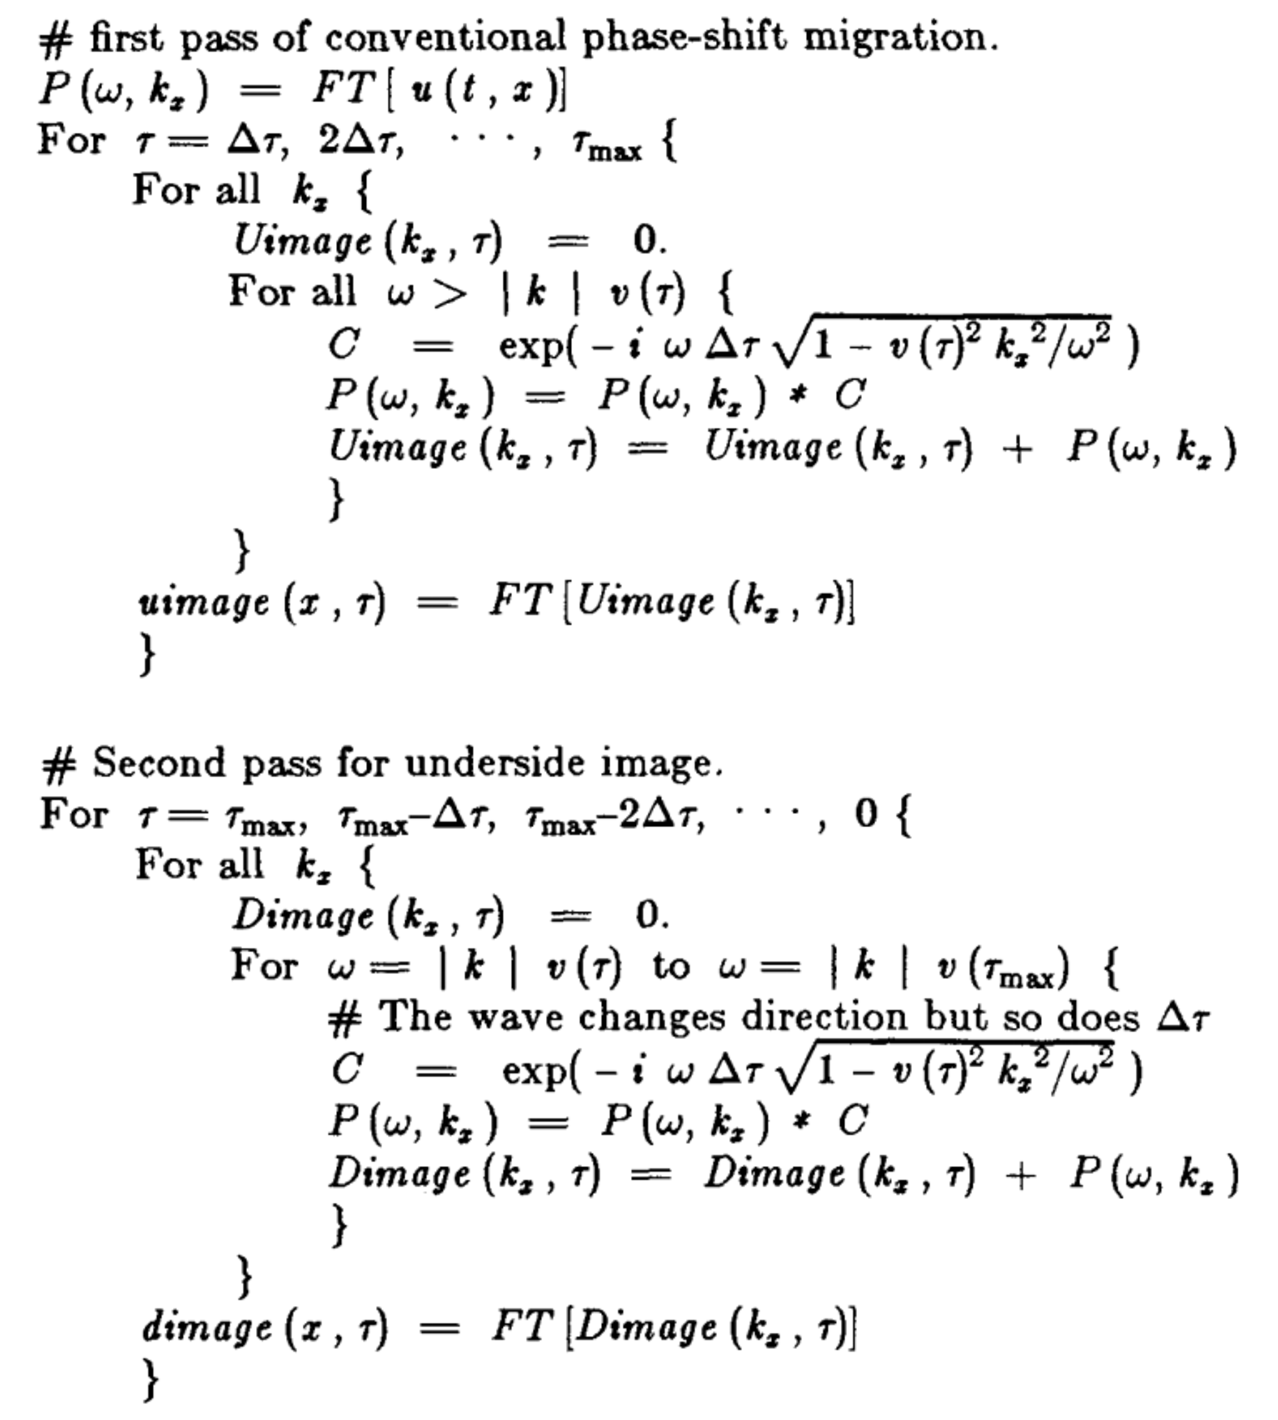
\includegraphics[width=0.65\textwidth]{crft/code1}
% \label{fig:crft/code1}
% \end{figure}
% \begin{figure}[H]
% \centering
% 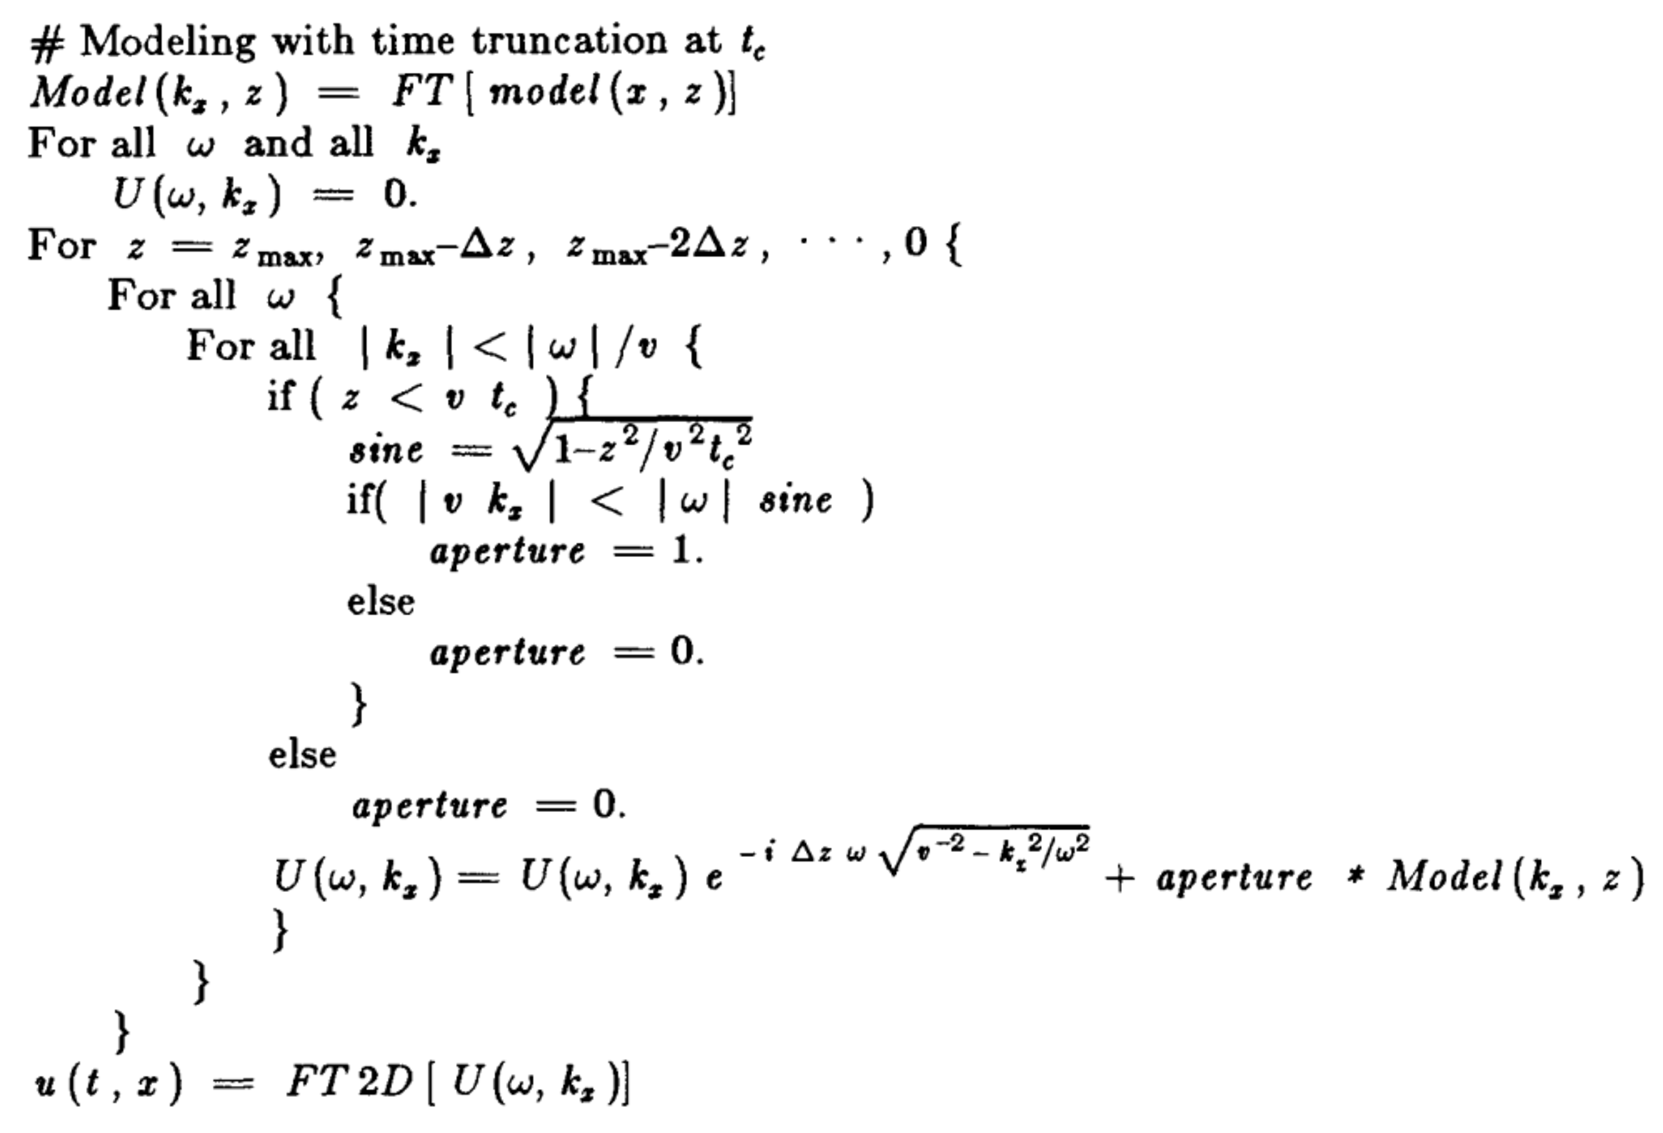
\includegraphics[width=0.65\textwidth]{crft/code2}
% \label{fig:crft/code2}
% \end{figure}
% \begin{figure}[H]
% \centering
% 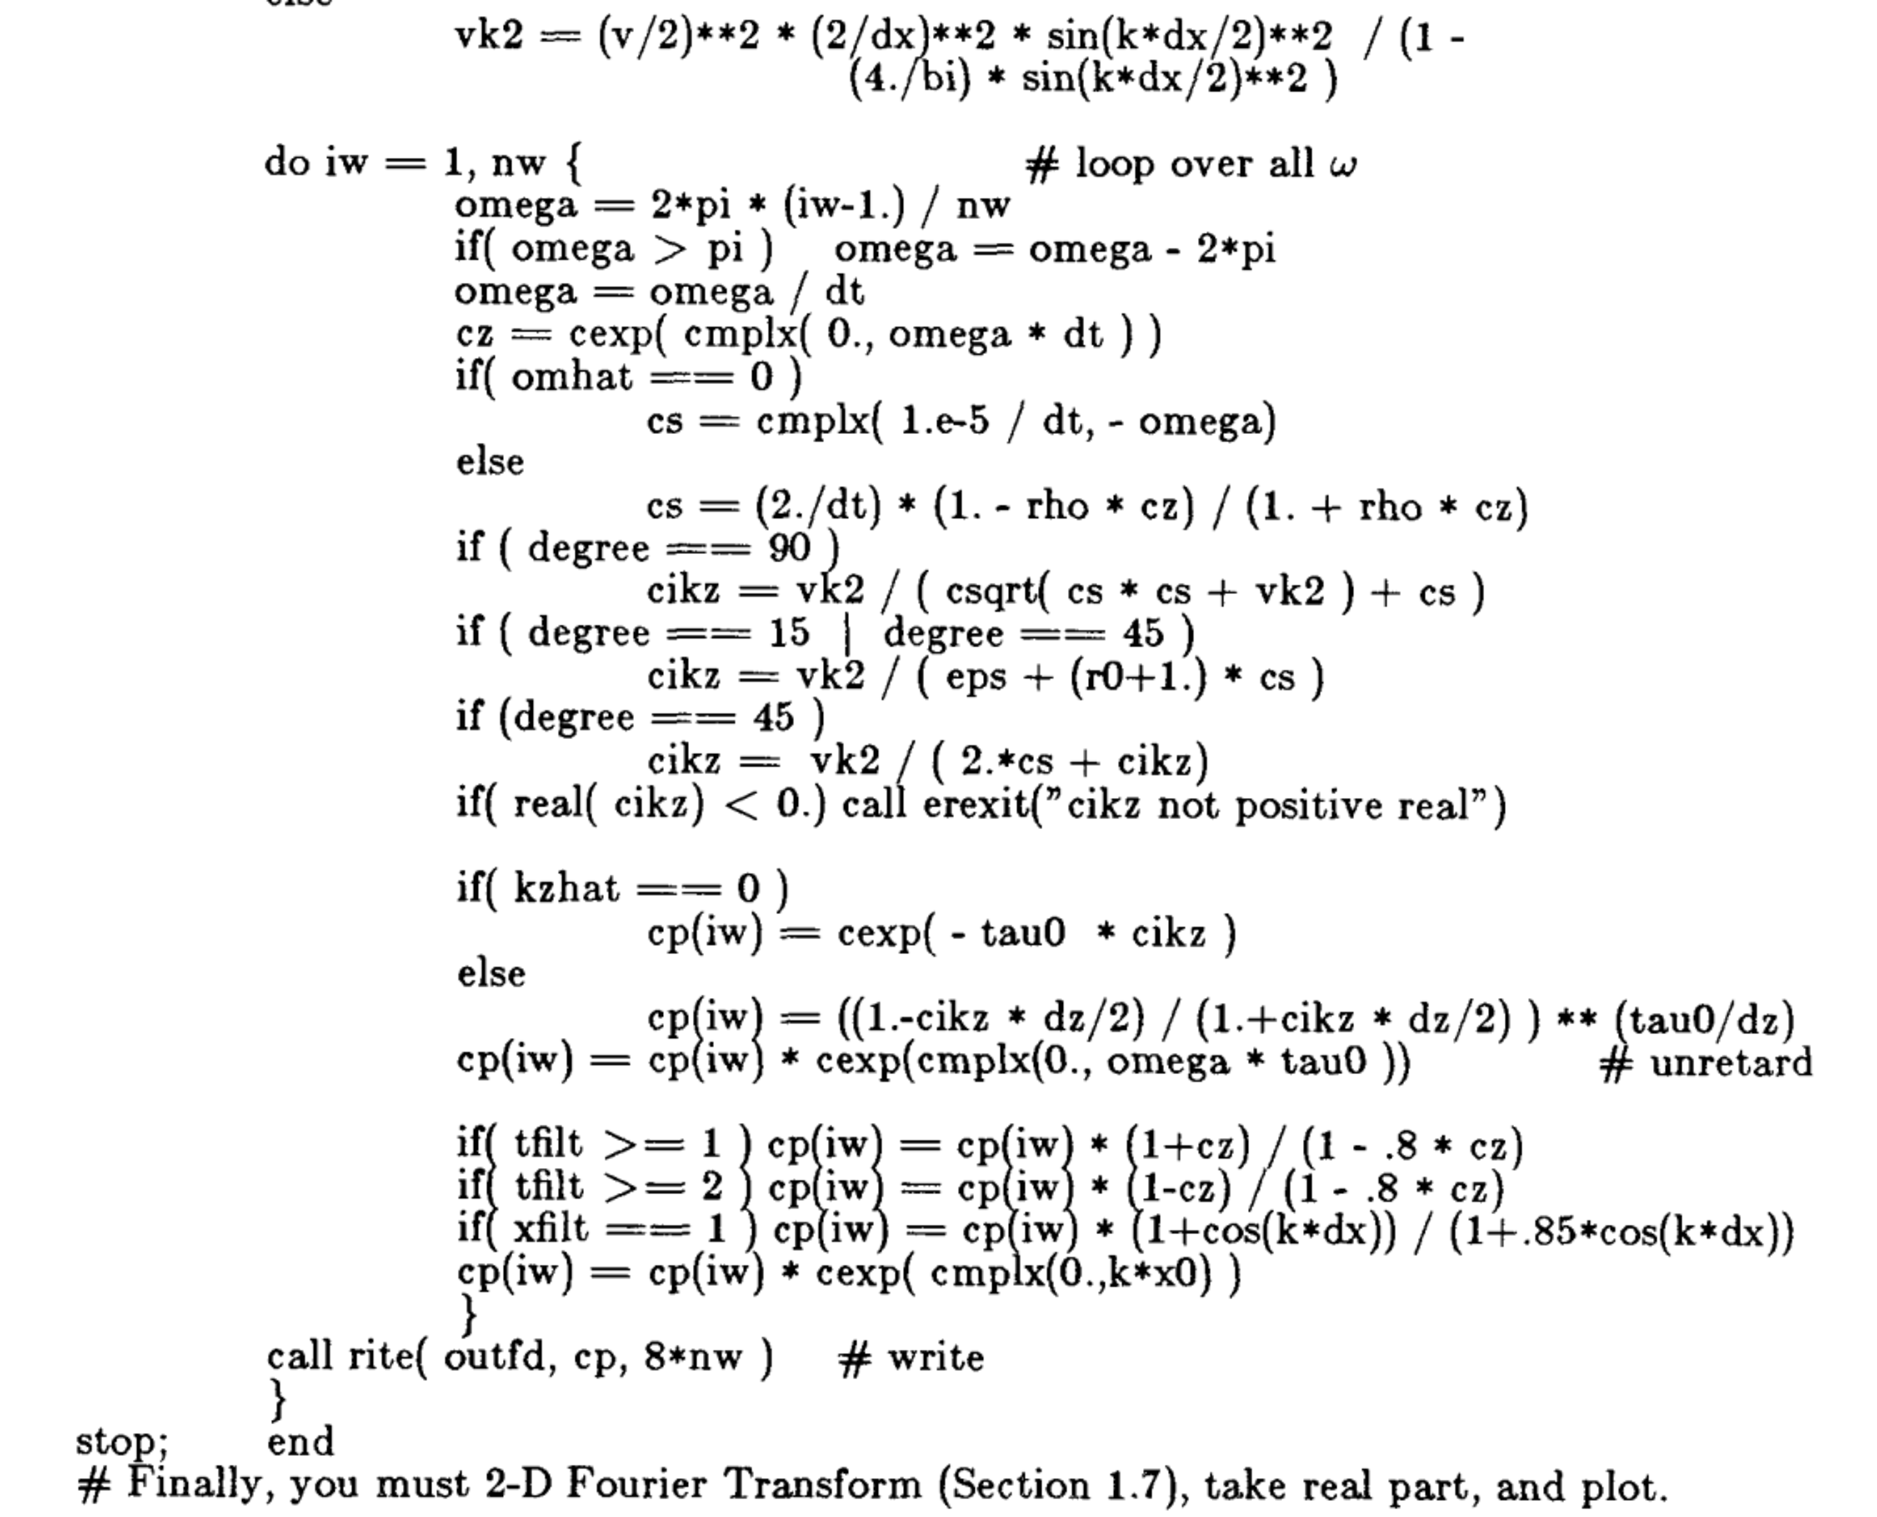
\includegraphics[width=0.65\textwidth]{crft/code3}
% \label{fig:crft/code3}
% \end{figure}

% 本书内有22个图件是由这个程序作出的,不同图件所采用的不同输入参量列表如下:
% \begin{table}[!ht]
% \centering
% \ttfamily
% \small
% \begin{tabularx}{\textwidth}{|Y|Y|}
% \hline
% 节号与图号 & 缺省参量 \\
% \hline
% 1.3-6a & tfilt=0 \\
% \hline
% 1.3-6b & \\
% \hline
% 2.0-1a & \\
% \hline
% 2.0-1b & $\hat{\omega}$ \\
% \hline
% 4.0-1a & $\hat{\omega},v=2.0, xf=.5, xfilt=0$ \\
% \hline
% 4.0-1b & $\hat{\omega},v=2.0, xf=.5 $ \\
% \hline
% 4.1-4a & 15°\\
% \hline
% 4.1-4b & $15^{\circ},\epsilon=1$\\
% \hline
% 4.1-5a & $45^{\circ},tf=.2$\\
% \hline
% 4.1-5b & $45^\circ, tf=.2, \epsilon=1$ \\
% \hline
% 4.2-4 & $45^\circ, tf=.2, \hat{\omega}$\\
% \hline
% 4.3-4a & $v=2.0,90^\circ$\\
% \hline
% 4.3-4b & $v=2.0,15^{\circ},\hat{\omega},\hat{k_x},\hat{k_z}$\\
% \hline
% 4.3-6a & $\hat{k_x},\hat{\omega},b^{-1}=1000000.$\\
% \hline
% 4.3-6b & $\hat{k_x},\hat{\omega},b^{-1}=12.$\\
% \hline
% 4.3-6c & $\hat{k_x},\hat{\omega},b^{-1}=6.726$\\
% \hline
% 4.3-6d & $\hat{k_x},\hat{\omega},b^{-1}=6.$\\
% \hline
% 4.3-6e & $\hat{k_x},\hat{\omega},b^{-1}=5.$\\
% \hline
% 4.6-2a & \\
% \hline
% 4.6-2b & $\hat{\omega}$ \\
% \hline
% 4.7-1a & $\Delta z=.004,45^{\circ},tf=.3,\hat{\omega},\hat{k_x},\hat{k_z}$\\
% \hline
% 4.7-1b & $\Delta z=.012,45^{\circ},tf=.3,\hat{\omega},\hat{k_x},\hat{k_z}$\\
% \hline
% \end{tabularx}
% \end{table} 

% 据说使z网格加密就能改善精度,如果x与t均属于连续统(continuum
% )这种结果是不
% 可能发生的,不过由于可使x与t离散化,偶然能消掉误差的可能性倒是存在的。为检查一下
% 这种传说是否成立,我试着把$\Delta z$増大3倍(实际上,就是将沿旅行时间深度的增量増大
% 3倍),结果如图\ref{fig:dspr/bigdz}所示。你对这图有何想法?

% \begin{figure}[H]
% \centering
% 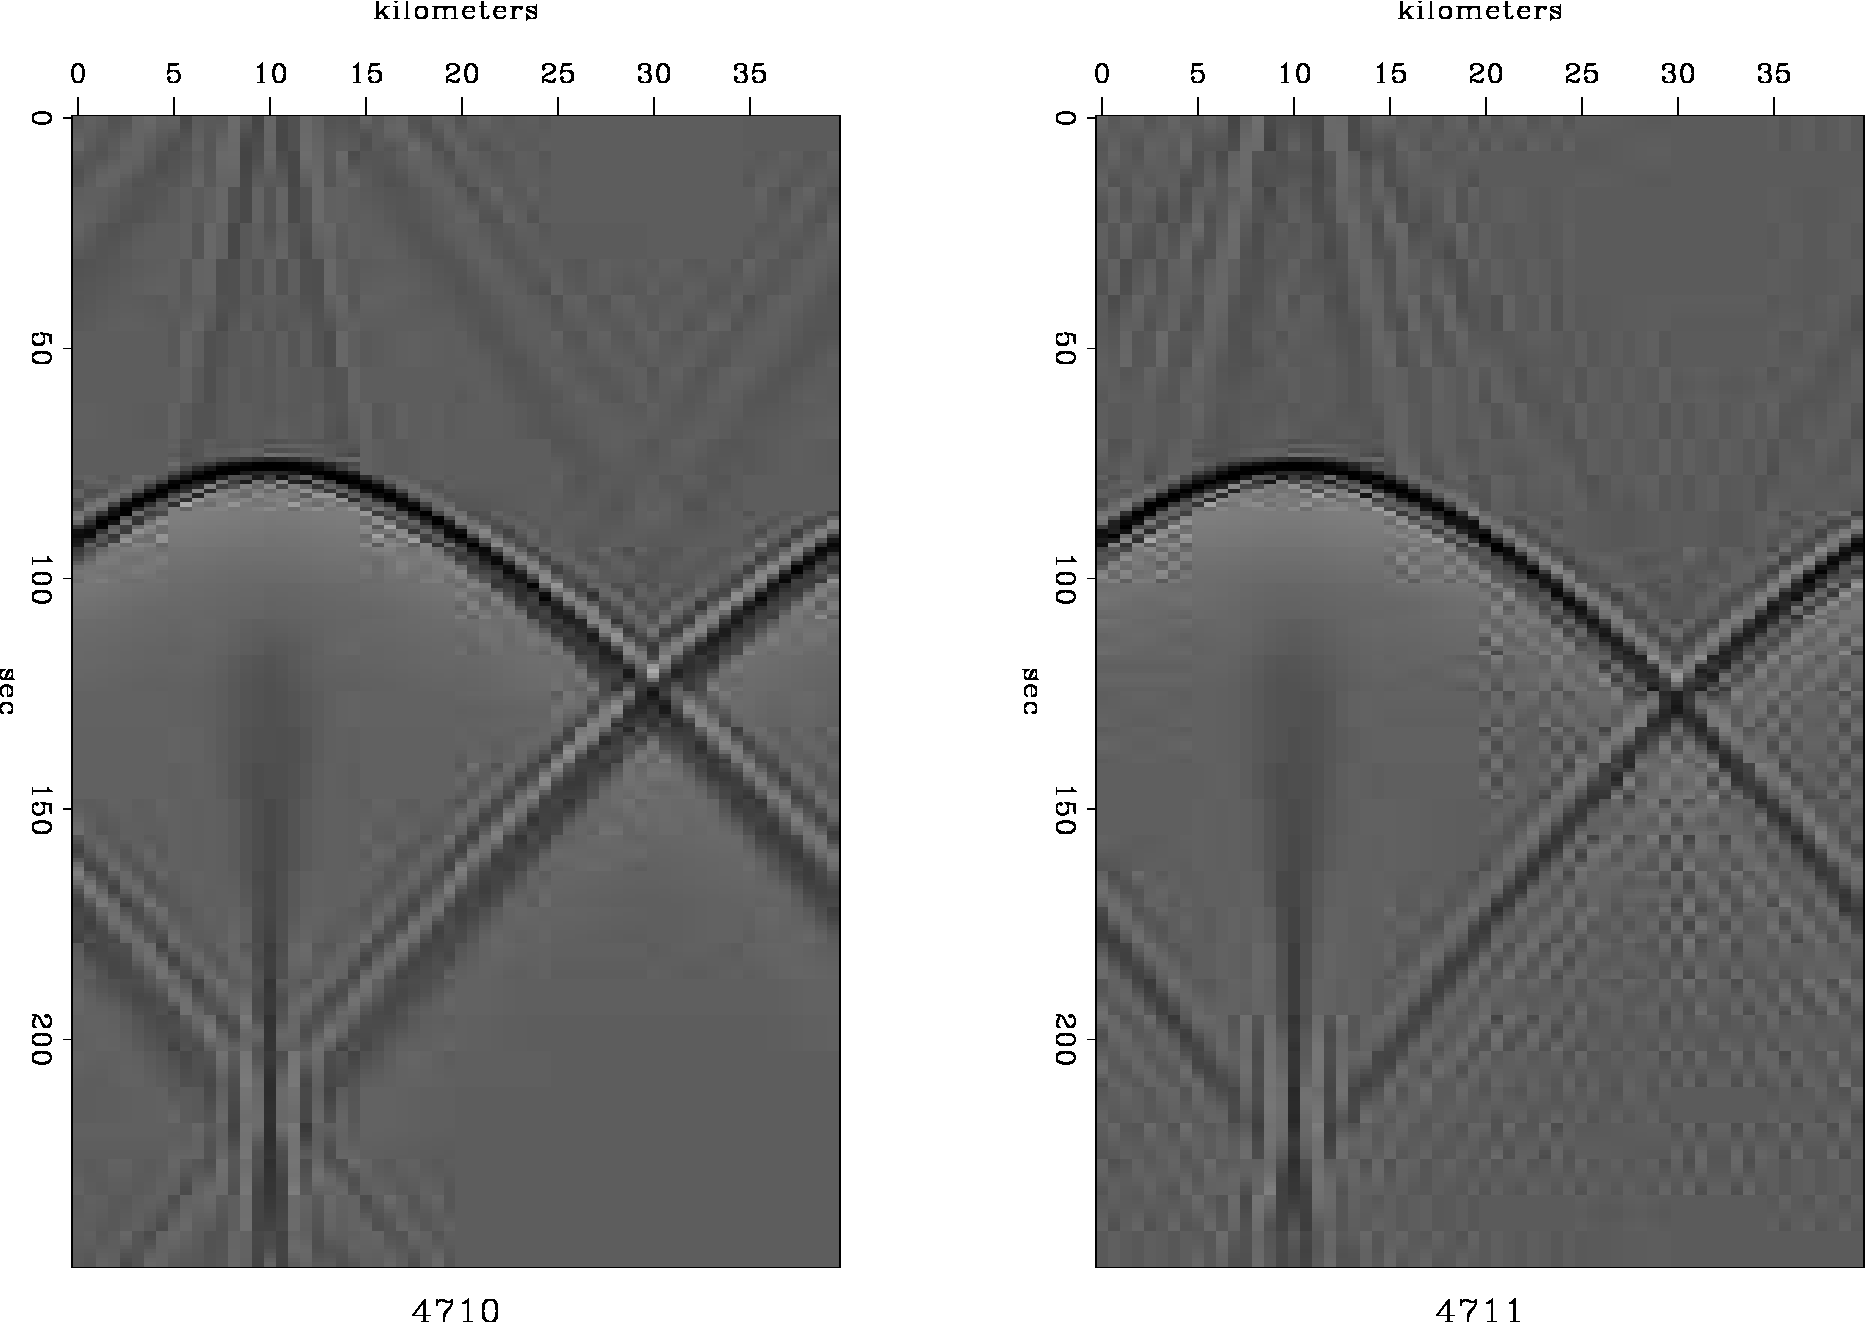
\includegraphics[width=0.65\textwidth]{dspr/bigdz}
% \caption[bigdz]{$(x,z,t)$空间中的45°点绕射,左图为$\Delta z=v\Delta t$,右图为$\Delta z=3v\Delta t$}
% \label{fig:dspr/bigdz}
% \end{figure}

% 这种分析看来就得到此结束了,由于Fourier分析是假设速度横向为恒定不变,分析受
% 到了限制。为处理这种问题,我们现在就转向下面一节有关处理技术这最后一讲。
